\documentclass[%
 reprint,
%superscriptaddress,
%groupedaddress,
%unsortedaddress,
%runinaddress,
%frontmatterverbose, 
%preprint,
%preprintnumbers,
%nofootinbib,
%nobibnotes,
%bibnotes,
 amsmath,amssymb,
 aps,
%pra,
%prb,
%rmp,
%prstab,
%prstper,
%floatfix,
]{revtex4-2}

\usepackage{graphicx}% Include figure files
\usepackage{dcolumn}% Align table columns on decimal point
\usepackage{bm}% bold math
\usepackage{physics}
\usepackage{cancel}
%\usepackage{hyperref}% add hypertext capabilities
%\usepackage[mathlines]{lineno}% Enable numbering of text and display math
%\linenumbers\relax % Commence numbering lines

%\usepackage[showframe,%Uncomment any one of the following lines to test 
%%scale=0.7, marginratio={1:1, 2:3}, ignoreall,% default settings
%%text={7in,10in},centering,
%%margin=1.5in,
%%total={6.5in,8.75in}, top=1.2in, left=0.9in, includefoot,
%%height=10in,a5paper,hmargin={3cm,0.8in},
%]{geometry}

\begin{document}

\preprint{APS/123-QED}

\title{Investigation of Finite Differencing Schemes Using\\the Linear Advection Equation}% Force line breaks with \\

\author{Evan Bluhm}
%  \altaffiliation[Also at ]{Physics Department, XYZ University.}%Lines break automatically or can be forced with \\
% \author{Second Author}%
%  \email{Second.Author@institution.edu}
% \affiliation{%
%  Authors' institution and/or address\\
%  This line break forced with \textbackslash\textbackslash
% }%


\date{May 14, 2021}% It is always \today, today,
             %  but any date may be explicitly specified
\begin{abstract}

We investigate the stability and accuracy of several explicit finite difference schemes, using the linear advection equation as the standard model for hyperbolic linear partial differential equations. Implementations of each scheme are applied to a model problem, and used to demonstrate the unconditional instability of the forward-time centered-space scheme, and the conditional stability of the simple upwind difference, Lax-Friedrichs, and Lax-Wendroff methods.
% % \begin{description}
% % \item[Usage]
% % Secondary publications and information retrieval purposes.
% % \item[Structure]
% % You may use the \texttt{description} environment to structure your abstract;
% % use the optional argument of the \verb+\item+ command to give the category of each item. 
% % \end{description}
\end{abstract}

%\keywords{Suggested keywords}%Use showkeys class option if keyword
                              %display desired
\maketitle

%\tableofcontents


\section{Introduction}

The study of ideal magnetohydrodynamics (MHD) requires solving a large system of partial differential equations, as outlined in detail in Appendix A. In Appendix B, we show that the ideal MHD system is hyperbolic, supporting several types of characteristic waves. Solving such a system analytically is rarely possible, and numerical schemes are required. Finite difference methods are a common technique for integrating partial differential equations.

There are a wide variety of finite difference schemes available, with widely varying accuracy, stability, and performance characteristics. In this paper, we focus on the forward-time centered-space method, a simple upwinding scheme, the Lax-Friedrichs method, and a Lax-Wendroff method. When investigating the properties of a numerical method, it is best to solve a model problem with a known exact solution, so that exact numerical errors are easy to calculate. The linear advection equation is the model equation for linear hyperbolic partial differential equations.

\section{Linear Advection Equation}

The one-dimensional linear advection equation a first-order hyperbolic partial differential equation:
\begin{equation}
\pdv{u}{t} + a \pdv{u}{x} = 0
\end{equation}
where $a$ is a constant characteristic speed. It is a useful model equation for investigating the stability and accuracy of numerical algorithms, as it has a very simple exact solution:
\begin{equation}
u(x - at) = \text{const.}
\end{equation}
That is, any initial state $u(x, t = 0)$ will propagate with speed $a$ in the positive direction if $a > 0$. This simple equation captures the wave-like nature of all linear hyperbolic partial differential equations. The exact solution of the linear advection equation has no dispersion, and no diffusion. When solving the advection equation using numerical methods, any diffusion and dispersion can be attributed solely to the properties of the numerical method itself.

% The linear advection equation has a single constant characteristic ($a$). This property can be used to validate the implementation of simple upwind differencing schemes, whose finite difference operators depend upon the sign of the wave velocity.

\section{Forward-Time, Centered-Space Differencing}

To obtain the forward-time, centered-space (FTCS) finite difference method, we replace temporal derivatives with forward differences, and spatial derivatives with centered differences. Using the notation $u_j^n$ to denote the value of $u$ at position $x = j\Delta x$ and time $t = n\Delta t$:
\begin{equation}
\pdv{u}{t} \rightarrow \frac{u_j ^{n+1} - u_j ^n}{\Delta t} \qquad \pdv{u}{x} \rightarrow \frac{u_{j+1} ^n - u_{j-1} ^n}{2 \Delta x}
\end{equation}
Applied to the linear advection equation, the time step operation is:
\begin{equation}
u_j ^{n+1} = u_j ^n - \frac{a \Delta t}{2 \Delta x} \left(u_{j+1} ^n - u_{j-1} ^n\right)
\end{equation}
A von Neumann stability analysis of this difference scheme finds that the method is unconditionally unstable, with amplification factor:
\begin{equation}
G \equiv \frac{|A^{n+1}|}{|A^n|} = \sqrt{1 + \left( \frac{ a \Delta t}{\Delta x} \right)^2 \sin ^2 (k \Delta x)} \geq 1
\end{equation}
where $A^n$ is the amplitude of an oscillatory mode at time step $n$, evolving under the FTCS scheme. To demonstrate the instability of the FTCS method, the results of a Python implementation of the algorithm are shown in Figure \ref{fig:ftcs-instability}. In this model, we initialize a short square pulse between $j=10$ and $j=20$ a grid of $201$ evenly spaced points. Using a time step of $\Delta t = 0.5$ and setting the advection speed to unity ($a = 1$), we step forward in time using the FTCS method until the square pulse reaches the rightmost grid point. We set Dirichlet boundary conditions at either side of the grid, such that $u_1 = u_M = 0$ at all times.

Note the scale of the y-axis in Figure \ref{fig:ftcs-instability}. The FTCS solution grows exponentially in time, along with the error. Since the square pulse contains all $k$, the modes with the largest growth will be those for which $\sin^2(k \Delta x) \approx 1$. For the model parameters, we expect an amplification factor
\begin{equation}
G = \sqrt{1 + \left( \frac{ a \Delta t}{\Delta x} \right)^2} \approx 1.41
\end{equation}
In the lower portion of Figure \ref{fig:ftcs-instability}, we plot the magnitude $A^n$ of the oscillations over time by taking the maximum value of $u$ in the FTCS solution. The regression of $\ln(A^n)$ vs $t$ gives an amplification factor of $G = 1.407$.

\begin{figure}
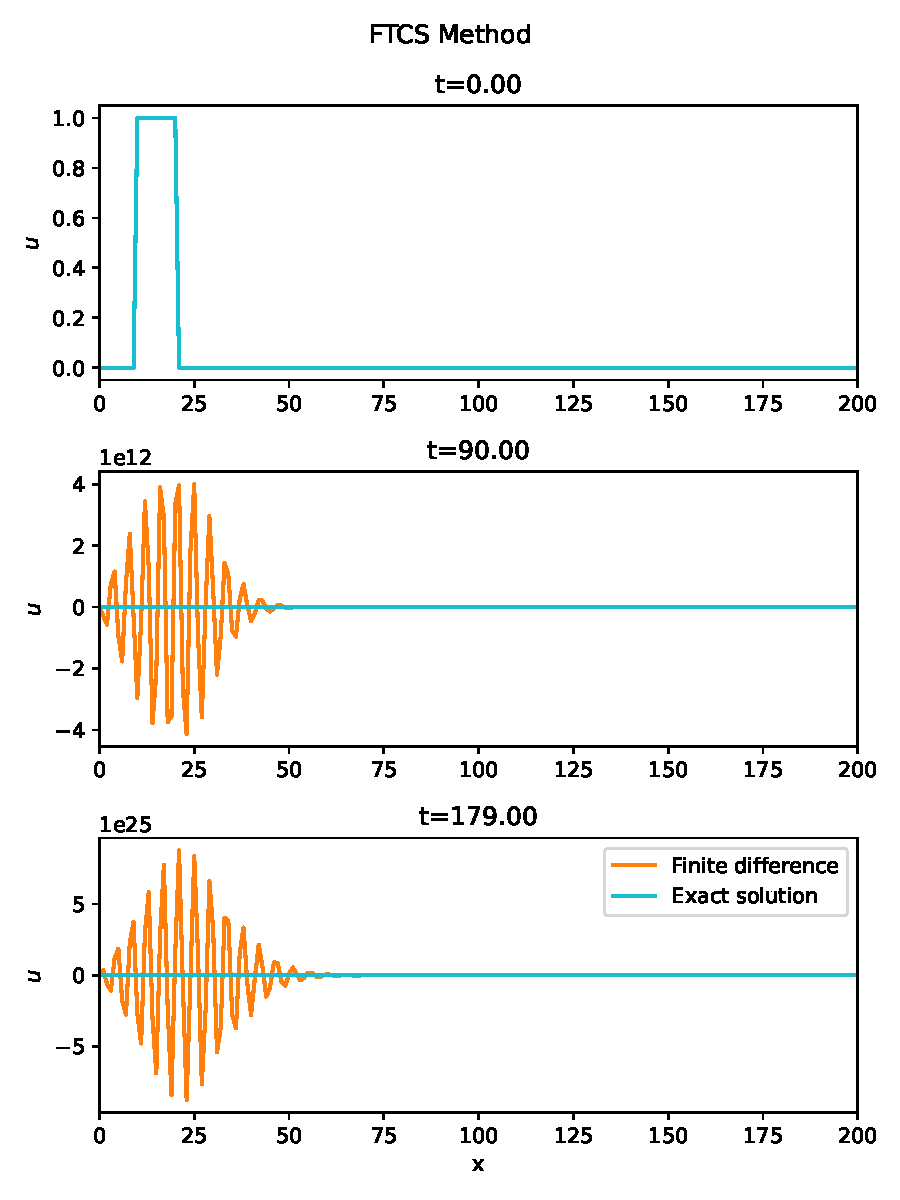
\includegraphics[width=0.9\linewidth]{proj2-1/snapshots-ftcs-instability.pdf}
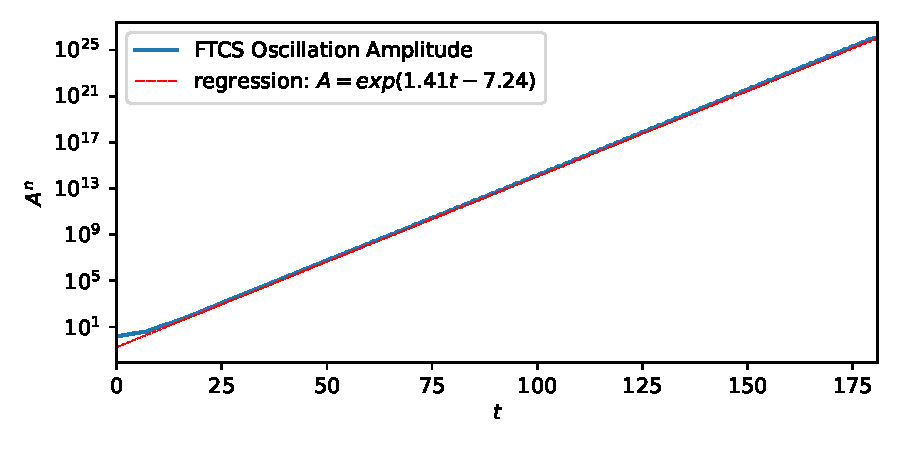
\includegraphics[width=0.9\linewidth]{proj2-1/ftcs-error-growth.pdf}
\caption{\label{fig:ftcs-instability}Snapshots of the evolution of a square pulse evolved using the FTCS numerical method, with parameters $a=1$, $\Delta t=0.5$, $\Delta x=1$, $M=201$. The exact solution is also shown. Below, the amplitude growth of the oscillations is plotted over time, revealing the exponential growth predicted by von Neumann analysis of the algorithm.}
\end{figure}

\section{Simple Upwind Difference}

One of the reasons the FTCS method performs so poorly with the advection equation is the unidirectional nature of the solution. There is only a single characteristic ($a$), which means that the domain of dependence at each point extends either forwards or backwards, but not both. The second-order centered spatial difference in the FTCS method makes use of both prior (``upwind'') and future (``downwind'') information to compute the gradient. This means that we will compute the gradient in the wrong location for any distribution that does not have a constant gradient. Instead, we can replace the second-order centered spatial difference with a first-order difference that does \emph{not} try to ``read the future'':
\begin{equation}
\pdv{u}{x} \approx \begin{cases} \frac{u_j ^n - u_{j-1} ^n}{\Delta x} \qquad  a > 0 \\
\frac{u_{j+1} ^n - u_{j} ^n}{\Delta x} \qquad  a < 0\end{cases}
\end{equation}
This leads to the simple upwind difference scheme:
\begin{equation}
u_j ^{n+1} = u_j ^n + \begin{cases} \frac{c \Delta t}{\Delta x} (u_{j-1} ^n - u_j ^n) \qquad a > 0 \\
\frac{c \Delta t}{\Delta x} (u_j ^n - u_{j-1} ^n) \qquad a < 0 \end{cases}
\end{equation}

\begin{figure}
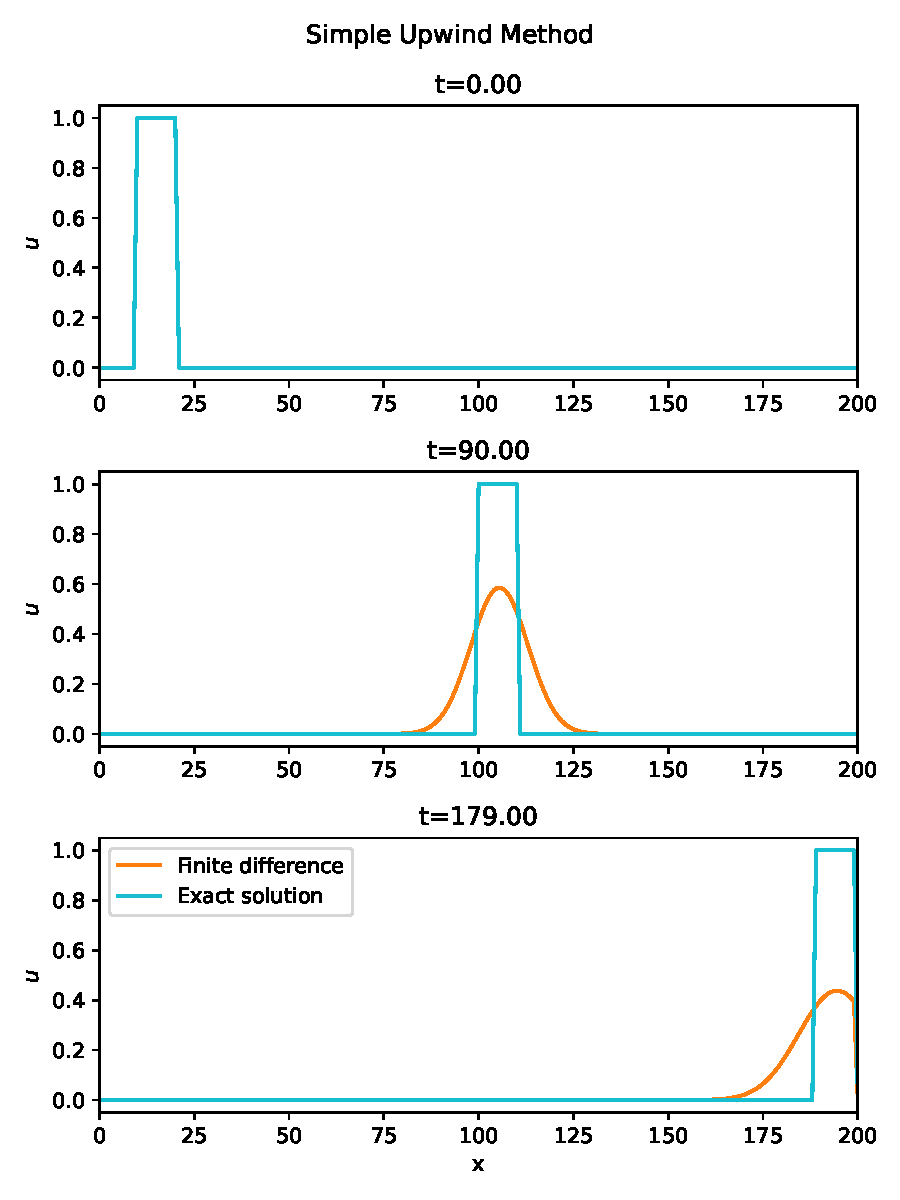
\includegraphics[width=0.9\linewidth]{proj2-1/snapshots-upwind.pdf}
\caption{\label{fig:upwind-snapshots}Evolution of the same pulse shown in Figure \ref{fig:ftcs-instability} with the FTCS method replaced by a simple upwind scheme. Model parameters are $a=1$, $\Delta t=0.5$, $\Delta x=1$, $M=201$. The method is stable, but a diffusive term has clearly been introduced.}
\end{figure}

The same von Neumann analysis for the simple upwind scheme gives an amplification factor:
\begin{equation}
G ^2 = 1 - 2 \frac{a \Delta t}{\Delta x} \left(1 - \frac{a \Delta t}{\Delta x} \right)(1 - \cos \theta)
\end{equation}
The term $\frac{a \Delta t}{\Delta x}$ is the Courant number, or CFL number $C$. For the simple upwind method to be stable, we require
\begin{equation}
0 \leq C \leq 1
\end{equation}
Our previous model parameters used $a = 1$, $\Delta x = 1$, and $\Delta t = 0.5$, giving $C = 0.5$, so the simple upwind method should produce stable results. Replacing the FTCS scheme with the simple upwind scheme and re-running our simulation with the same model parameters, we find that the upwind scheme is indeed stable, as shown in Figure \ref{fig:upwind-snapshots}.
We can see that we've also introduced a diffusive term. One way to see where this term comes from is to perform a truncation analysis by replacing the terms in our finite difference with their truncated Taylor expansions:
\begin{equation}
u_j ^{n+1} = u_j ^n + \partial _t u \Delta t + \frac{1}{2} \partial_{tt} u \Delta t^2 + \mathcal{O}(\Delta t^3)
\end{equation}
\begin{equation}
u_{j \pm 1} ^n = u_j ^n \pm \partial _x u \Delta x + \frac{1}{2} \partial_{xx} u \Delta x^2 + \mathcal{O}(\Delta x^3)
\end{equation}
Plugging these into the simple upwind finite difference and solving for our original PDE $\partial _t u + a \partial_x u$, we find that there is a first-order diffusion term:
\begin{equation}
\partial_t u + a \partial_x u = \frac{1}{2} u \Delta x (1 - C) \partial_{xx} u
\end{equation}
which contributes physical diffusion if $C < 1$, and instability if $C > 1$. Interestingly, when $C = 1$ we recover the exact PDE, and the simple upwind method perfectly solves the linear advection equation. This is nice, but not generally useful for higher-order differential equations with more than one characteristic.

\section{Lax Method}

Taking some inspiration from the simple upwind difference scheme, we found that adding a diffusive term helped to smooth over oscillatory error terms and stabilize the method, at the cost of accuracy. The Lax-Friedrichs method deliberately adds diffusion by taking a spatial average when calculating the time step:
\begin{equation}
u_j ^n \rightarrow \frac{u_{j+1} ^n + u_{j-1} ^n}{2}
\end{equation}
giving the modified scheme:
\begin{equation}
u_j ^{n+1} = \frac{1}{2} (1 + C) u_{j-1} ^n + \frac{1}{2} (1 - C) u_{j+1} ^n
\end{equation}
A von Neumann stability analysis finds an amplification factor of:
\begin{equation}
G = \sqrt{1 - \left[ 1 - C^2 \right] \sin ^2 ( k \Delta x)}
\end{equation}
so we must satisfy the Courant condition for the Lax-Friedrichs algorithm to be stable:
\begin{equation}
|C| = \left| \frac{a \Delta t}{\Delta x} \right| \leq 1 
\end{equation}

Running our previous simulation with the same model parameters ($C = 0.5$), we see the results shown in Figure \ref{fig:snapshots-lax}. The short-wavelength oscillations that were the cause of instability in the FTCS scheme are still present, but the spatial averaging has damped them. If we re-write the Lax time step, we can see the coefficient of the diffusive term:
\begin{eqnarray*}
u_j ^{n+1} & = & \frac{u_{j+1} ^n + u_{j-1} ^n}{2} - \frac{a \Delta t}{\Delta x} \left( \frac{u_{j+1} ^n - u_{j - 1} ^n}{2} \right) \\
& = & u_j ^n - \frac{a \Delta t}{\Delta x} \frac{u_{j+1} ^n - u_{j - 1} ^n}{2} + \frac{u_{j+1} ^n - 2 u_j ^n + u_{j-1} ^n}{2}
\end{eqnarray*}
which is a finite difference approximation of the modified PDE:
\begin{equation}
\pdv{u}{t} + a \pdv{u}{x} = \frac{\Delta x ^2}{\Delta t} \pdv{^2 u}{x ^2}
\end{equation}
So the artificial diffusive term carries a viscosity $\Delta x ^2 / \Delta t$. In the limit $\Delta x \rightarrow 0$, we converge to the original PDE, but only as long as $\Delta x ^2$ shrinks faster than $\Delta t$. For large characteristic speeds $a$, we require an extremely finely spaced grid to meet the Courant condition without introducing unacceptable amounts of diffusion.

\begin{figure}
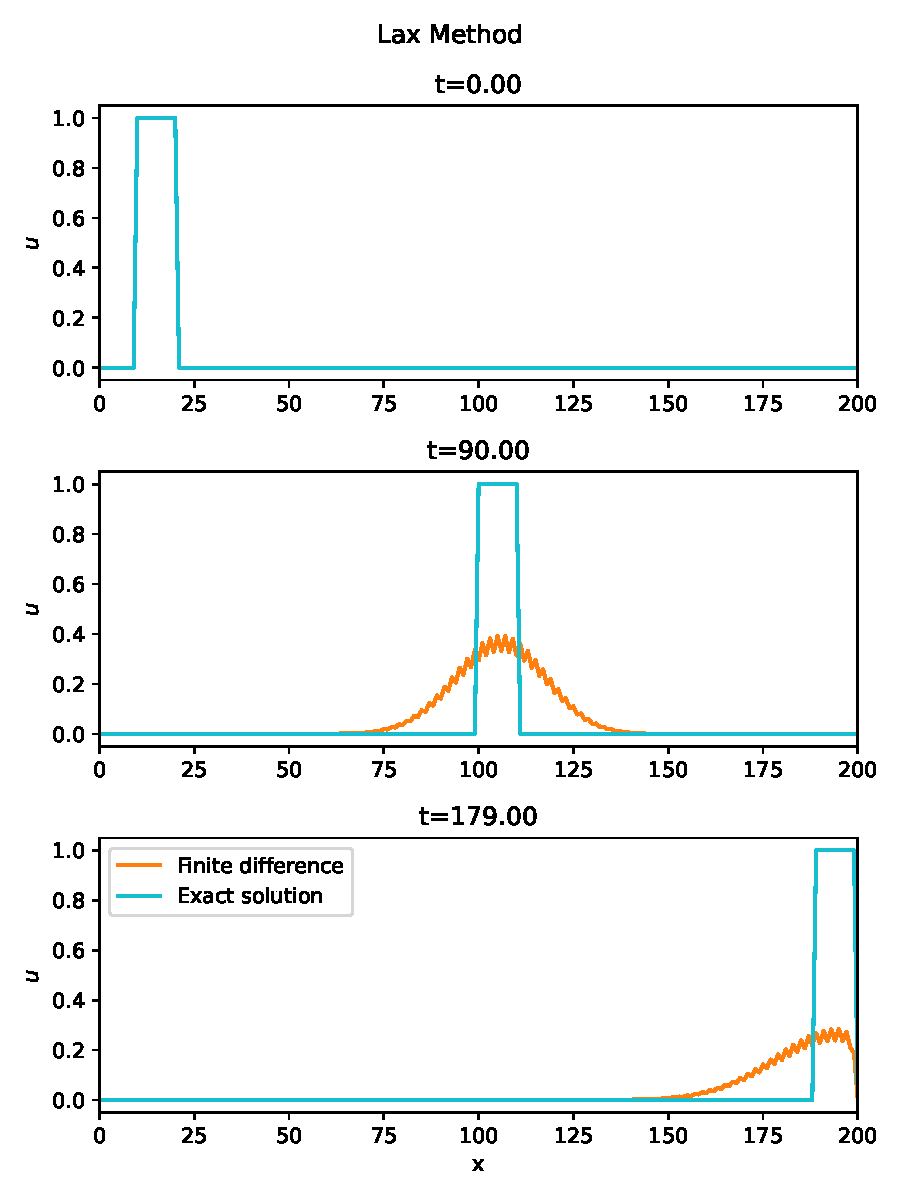
\includegraphics[width=0.9\linewidth]{proj2-1/snapshots-lax.pdf}
\caption{\label{fig:snapshots-lax}Evolution of a square pulse using the Lax-Friedrichs scheme. Model parameters are $a=1$, $\Delta t=0.5$, $\Delta x=1$, $M=201$. The method is stable, but more diffusive than the simple upwind method. The oscillations arising from the FTCS instability are visible, but sufficiently damped to remove the instability.}
\end{figure}


\begin{figure}[h]
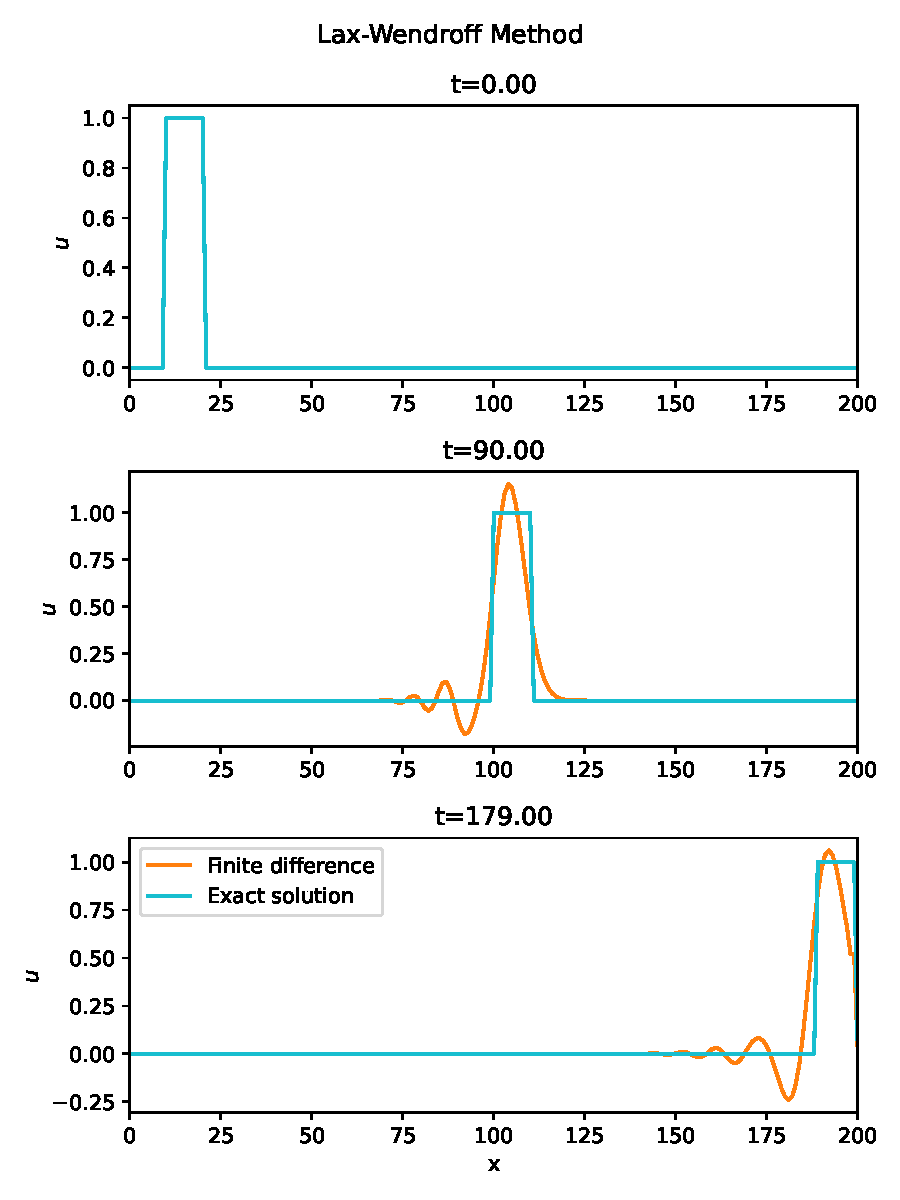
\includegraphics[width=0.9\linewidth]{proj2-1/snapshots-lax-wendroff.pdf}
\caption{\label{fig:snapshots-lax-wendroff}Evolution of a square pulse using the Lax-Wendroff scheme. Model parameters are $a=1$, $\Delta t=0.5$, $\Delta x=1$, $M=201$. Compared with the Lax and simple upwind methods, there is far less diffusive smearing of the solution. The diffusion in the Lax-Wendroff scheme is just sufficient to stabilize oscillations.}
\end{figure}

\section{Lax-Wendroff Method}

The Lax-Wendroff method is similar to the Lax-Friedrichs method, as it also adds a diffusive term to the FTCS algorithm, but with a different viscosity. The standard Lax-Wendroff two-step method is composed of two steps. First we predict the value of $u^{n \pm 1/2} _{j \pm 1/2}$, then we use that prediction to compute the appropriately-centered gradient. The first step, using the Lax scheme, reads:
\begin{equation*}
u_{j + 1/2} ^{n + 1/2} = \frac{1}{2} \left( u_{j + 1} ^n + u_j ^n \right) - \frac{a \Delta t}{2 \Delta x} \left( u_{j+1} ^n - u_j ^n \right)
\end{equation*}
\begin{equation*}
u_{j + 1/2} ^{n + 1/2} = \frac{1}{2} \left( u_{j + 1} ^n + u_j ^n \right) - \frac{a \Delta t}{2 \Delta x} \left( u_{j+1} ^n - u_j ^n \right)
\end{equation*}
and the second step, using a half step of the leapfrog scheme, is
\begin{equation}
u_j ^{n+1} = u_j ^n - \frac{a \Delta t}{\Delta x} \left( u_{j + 1/2} ^{n + 1/2} - u_{j - 1/2} ^{n + 1/2} \right)
\end{equation}
Combining the two steps for the linear advection equation, we can see the diffusive term and associated viscosity:
\begin{eqnarray*}
u_j ^{n+1} & = & u_j ^n - \frac{a \Delta t}{2 \Delta x} \left( u_{j+1} ^n - u_{j-1} \right) \\
& & + \frac{ a^2 \Delta t ^2}{2 \Delta x ^2} \left( u_{j + 1} ^n - 2 u_j ^n + u_{j - 1} ^n \right)
\end{eqnarray*}
this is a finite difference approximation of the PDE:
\begin{equation}
\pdv{u}{t} + a \pdv{u}{x} = \frac{a^2 \Delta t}{2} \pdv{^2 u }{x^2}
\end{equation}
Now the strength of the diffusion term is no longer related to the grid spacing, so we are free to raise the time step as long as the CFL condition is met. The von Neumann stability analysis yields an amplification factor:
\begin{equation}
G ^2 = 1 - C^2 (1 - C^2) \left[1 - \cos ^2 (k \Delta x) \right]
\end{equation}
which is less than 1 as long as $C \leq 1$. For $C = 1$, the dissipation disappears entirely and we exactly solve the linear advection equation, as was the case for the simple upwind method.

Figure \ref{fig:snapshots-lax-wendroff} shows the application of the Lax-Wendroff method with our model parameters. We can see that the excessive diffusion that was present in the simple upwind and Lax-Friedrichs schemes is no longer as intense. The method is stable for our model parameters, since $C = 0.5$. Unlike the Lax-Friedrichs scheme, the Lax-Wendroff scheme converges to the mode PDE as $\Delta t \rightarrow 0$, without restrictions on the grid spacing, allowing us to capture faster-propagating characteristics without the need for expensively large grids. Taylor expansion of the finite difference expression shows that Lax-Wendroff is second-order accurate in both space and time. These properties make it the method of choice for a wide variety of applications.

\section{Conclusions}
The model system investigated here reveals various pitfalls of finite difference methods. Stability of a method is an important consideration, which can place restrictions on the time step and grid spacing based on the characteristic speeds of the system. Instabilities arise as growing oscillatory terms, as predicted by von Neumann analysis. The methods given here show several ways to add numerical diffusion and smooth out the oscillations, creating stability.


\onecolumngrid

\pagebreak

\appendix

\section{Conservative Form of Ideal MHD Equations}

Starting from a set of non-conservative equations for ideal MHD, we wish to re-cast the system of equations in a conservative form:
\begin{equation}
\pdv{}{t} \vec Q + \div \vec F = 0
\end{equation}

To begin with, the non-conservative continuity equation for ideal MHD is:
\begin{equation}
\pdv{\rho}{t} + \vec v \cdot \grad \rho = - \rho \div \vec v
\end{equation}
where $\rho$ is the single-fluid mass density, and $\vec v$ is the center-of-mass velocity. Application of the product rule $\div (a \vec b) = a \div \vec b + (\grad a) \cdot \vec b$ gives
\begin{eqnarray}
0 & = & \pdv{\rho}{t} + \vec v \cdot \grad \rho + \rho \div \vec v \\
& = & \pdv{\rho}{t} + \div (\rho \vec v)
\end{eqnarray}
Moving on to the non-conservative form of the momentum equation, we have
\begin{equation}
0 = \rho \left( \pdv{\vec v}{t} + \vec v \cdot \grad v \right) + \grad p - \vec j \cross \vec B
\end{equation}
where $\vec B$ is the magnetic field, $\vec j$ is the current density, and $p$ is the plasma pressure. Expanding the first term and using the conservative form of the continuity equation,
\begin{eqnarray}
\rho \pdv{\vec v}{t} & = & \pdv{(\rho \vec v)}{t} - \vec v \pdv{\rho}{t} \\
& = & \pdv{(\rho \vec v)}{t} + \vec v \left( \div (\rho \vec v) \right)
\end{eqnarray}
Substituting back into the momentum equation,
\begin{eqnarray}
0 & = & \pdv{(\rho \vec v)}{t} + \vec v \div (\rho \vec v) + \rho \vec v \cdot \grad v + \grad p - \vec j \cross \vec B \\
& = & \pdv{(\rho \vec v)}{t} + \div (\rho \vec v \vec v) + \grad p - \vec j \cross \vec B
\end{eqnarray}
Using Ampere's law to expand $\vec j$,
\begin{eqnarray}
\vec j \cross \vec B & = & \frac{1}{\mu_0} (\curl \vec B) \cross \vec B \\
& = & \frac{1}{\mu_0} (\vec B \cdot \grad) \vec B -  \grad \frac{B^2}{2 \mu_0} \\
& = & \frac{1}{\mu_0} \div (\vec B \vec B) - \vec B (\div \vec B) - \grad \frac{B^2}{2 \mu_0} \\
& = & \frac{1}{\mu_0} \div (\vec B \vec B) - \grad \frac{B^2}{2 \mu_0} \qquad (\div \vec B = 0)
\end{eqnarray}
Finally, we can put the momentum equation into conservative form
\begin{eqnarray}
0 & = & \pdv{(\rho \vec v)}{t} + \div (\rho \vec v \vec v) + \grad p - \left[\frac{1}{\mu_0} \div (\vec B \vec B) - \grad \frac{B^2}{2 \mu_0} \right] \\
& = & \pdv{(\rho \vec v)}{t} + \div (\rho \vec v \vec v) + \div \frac{\vec B \vec B}{\mu_0} + \grad \left( p + \frac{B^2}{2 \mu_0} \right) \\
& = & \pdv{(\rho \vec v)}{t} + \div \left[ \rho \vec v \vec v - \frac{\vec B \vec B}{\mu_0} + \left( p + \frac{B^2}{2\mu_0} \right) \vec{1} \right]
\end{eqnarray}
For ideal MHD, we treat the fluid as a perfect conductor, so that
\begin{equation}
\vec E = - \vec v \cross \vec B
\end{equation}
Faraday's law gives
\begin{eqnarray}
\pdv{\vec B}{t} & = &  - \curl \vec E\\
& = & \curl (\vec v \cross \vec B) \\
& = & \div ( \vec B \vec v - \vec v \vec B)
\end{eqnarray}
So we arrive at an equation for $\vec B$ in conservative form:
\begin{equation}
\pdv{\vec B}{t} + \div (\vec v \vec B - \vec B \vec v) = 0
\end{equation}

Finally, we need a conservation law for the energy density $e$ in conservative form.
\begin{equation}
e = \frac{p}{\gamma - 1} + \frac{\rho v^2}{2} + \frac{B^2}{2 \mu_0}
\end{equation}
We can get there by taking the dot product of our momentum equation with $\vec v$:
\begin{equation}
\vec v \cdot \rho \left( \pdv{\vec v}{t} + \vec v \cdot \grad \vec v\right) = \vec v \cdot \left[ \vec j \cross \vec B - \grad p \right]
\end{equation}
Starting from the left, we can use our continuity equation to write the left-hand side as
\begin{eqnarray}
\vec v \cdot \rho \left( \pdv{\vec v}{t} + \vec v \cdot \grad \vec v\right) & = & \frac{1}{2} \rho \left( \pdv{v^2}{t} + \vec v \cdot \grad v^2 \right) \\
& = & \pdv{}{t} \left( \frac{\rho v^2}{2} \right) - \frac{v^2}{2} \pdv{\rho}{t} + \frac{1}{2} \rho \vec v \cdot \grad v^2 \\
& = & \pdv{}{t} \left( \frac{\rho v^2}{2} \right) + \frac{v^2}{2} \div (\rho \vec v) + \frac{1}{2} \rho \vec v \cdot \grad \vec v \\
& = & \pdv{}{t} \left( \frac{\rho v^2}{2} \right) + \div \left( \frac{\rho v^2}{2} \vec v \right)
\end{eqnarray}
So we now have:
\begin{equation}
\pdv{}{t} \left( \frac{\rho v^2}{2} \right) + \div \left( \frac{\rho v^2}{2} \vec v \right) = \vec v \cdot \left[ \vec j \cross \vec B - \grad p \right]
\end{equation}
To expand the $\vec j \cross \vec B$ term, we once again use Ampere's law to expand $\vec j$:
\begin{eqnarray}
\vec v \cdot ( \vec j \cross \vec B) & = & \frac{1}{\mu_0}\vec v \cdot \left( \curl \vec B \right) \cross \vec B \\
& = & - \frac{1}{\mu_0}(\vec v \cross \vec B) \cdot (\curl \vec B) \\
& = & \frac{1}{\mu_0} \vec E \cdot (\curl \vec B) \qquad \qquad (\vec E = - \vec v \cross \vec B) \\
& = & \frac{1}{\mu_0} \vec B \cdot (\curl \vec E) - \frac{1}{\mu_0} \div (\vec E \cross \vec B)
\end{eqnarray}
Using Faraday's law, we can extract $\pdv{\vec B}{t}$:
\begin{eqnarray}
\vec v \cdot (\vec j \cross \vec B) & = & \frac{1}{\mu_0} \vec B \cdot (\curl \vec E) - \frac{1}{\mu_0} \div (\vec E \cross \vec B) \\
& = & - \frac{1}{\mu_0} \vec B \cdot \left(\pdv{\vec B}{t} \right) - \frac{1}{\mu_0} \div (\vec E \cross \vec B) \\
& = & - \pdv{}{t} \left( \frac{B^2}{2 \mu_0} \right) - \frac{1}{\mu_0} \div (\vec E \cross \vec B) \\
& = & - \pdv{}{t} \left( \frac{B^2}{2 \mu_0} \right) - \frac{1}{\mu_0}\div \left( (- \vec v \cross \vec B) \cross \vec B \right) \\
& = & - \pdv{}{t} \left( \frac{B^2}{2 \mu_0} \right) - \frac{1}{\mu_0} \div \left( B^2 \vec v - (\vec B \cdot \vec v) \vec B \right) \\
& = & - \pdv{}{t} \left( \frac{B^2}{2 \mu_0} \right) - \div \left( \frac{B^2}{\mu_0} \vec v - \frac{\vec B \cdot \vec v}{\mu_0} \vec B \right)
\end{eqnarray}
And moving on to the $\vec v \cdot \grad p$ term, we use the adiabatic equation of state:
\begin{equation}
\pdv{p}{t} + ( \vec v \cdot \grad p) = - \gamma p \div \vec v
\end{equation}
Extracting $\vec v \cdot \grad p$,
\begin{eqnarray}
\pdv{p}{t} + ( \vec v \cdot \grad p) & = & - \gamma p \div \vec v \\
\pdv{p}{t} + ( \vec v \cdot \grad p) & = & - \gamma \div (p \vec v) + \gamma(\vec v \cdot \grad p) \\
\vec v \cdot \grad p & = & \frac{1}{\gamma - 1} \pdv{p}{t}  + \frac{\gamma}{\gamma - 1} \div (p \vec v)
\end{eqnarray}
Combining all three together, and using:
\begin{equation}
\frac{\gamma}{\gamma - 1} p = e + p - \frac{\rho v^2}{2} - \frac{B^2}{2 \mu_0}
\end{equation}
we finally arrive at the conservative form of the energy equation:
\begin{eqnarray}
\vec v \cdot \rho \left( \pdv{\vec v}{t} + \vec v \cdot \grad \vec v\right) & = & \vec v \cdot (\vec j \cross \vec B) -  \vec v \cdot \grad p \\
\pdv{}{t} \left( \frac{\rho v^2}{2} \right) + \div \left( \frac{\rho v^2}{2} \vec v \right) & = & - \pdv{}{t} \left( \frac{B^2}{2 \mu_0} \right) - \div \left( \frac{B^2}{\mu_0} \vec v - \frac{\vec B \cdot \vec v}{\mu_0} \vec B \right) - \frac{1}{\gamma - 1} \pdv{p}{t}  - \frac{\gamma}{\gamma - 1} \div (p \vec v) \\
\pdv{}{t} \underbrace{\left( \frac{\rho v^2}{2} + \frac{p}{\gamma - 1} + \frac{B^2}{2 \mu_0} \right)}_{= e} & = & - \div \left[ \left( \frac{\rho v^2}{2} + \frac{\gamma}{\gamma - 1} p + \frac{B^2}{\mu_0} \right) \vec v - \frac{\vec B \cdot \vec v}{\mu_0} \vec B \right] \\
\pdv{e}{t} & = & - \div \left[ \left(e + p + \frac{B^2}{2 \mu_0} \right) \vec v - \frac{\vec B \cdot \vec v}{\mu_0} \vec B \right]
\end{eqnarray}

\section{Differential Equation Type of 1D Ideal MHD}


The conservative form of the ideal MHD equations can be expressed as a matrix equation:
\begin{equation}
\pdv{\vec Q}{t} + \div \vec{T} = 0
\end{equation}
where
\begin{equation}
\vec Q = \begin{bmatrix}
\rho &
\rho v_x &
\rho v_y &
\rho v_z &
B_x &
B_y &
B_z &
e
\end{bmatrix}^\top
\end{equation}
and
\begin{equation}
\vec T = \begin{bmatrix}
\rho v_x & \rho v_y & \rho v_z \\
\rho v_x^2 + p + \frac{B^2}{2 \mu_0} - \frac{B_x ^2}{\mu_0} & \rho v_x v_y - \frac{B_x B_y}{\mu_0} & \rho v_x v_z - \frac{B_x B_z}{\mu_0} \\
\rho v_y v_x - \frac{B_y B_x}{\mu_0} & \rho v_y ^2 + p + \frac{B^2}{2 \mu_0} - \frac{B_y ^2}{\mu_0} & \rho v_y v_z - \frac{B_y B_z}{\mu_0} \\
\rho v_z v_x - \frac{B_x B_z}{\mu_0} & \rho v_z v_y - \frac{B_z B_y}{\mu_0} & \rho v_z ^2 + p + \frac{B^2}{2 \mu_0} - \frac{B_z ^2}{\mu_0} \\
0 & B_x v_y - v_x B_y & B_x v_z - v_x B_z  \\
B_y v_x - v_y B_x  & 0 & B_y v_z - v_y B_z  \\
B_z v_x - v_z B_x & B_z v_y - v_z B_y & 0 \\
\left( e + p + \frac{B^2}{2 \mu_0} \right) v_x - \frac{\vec B \cdot \vec v}{\mu_0} B_x & \left( e + p + \frac{B^2}{2 \mu_0} \right) v_y - \frac{\vec B \cdot \vec v}{\mu_0} B_y & \left( e + p + \frac{B^2}{2 \mu_0} \right) v_z - \frac{\vec B \cdot \vec v}{\mu_0} B_z
\end{bmatrix} ^ \top
\end{equation}

To determine whether the ideal MHD system of equations is elliptic, parabolic, or hyperbolic, we need to determine the eigenvalues of the flux Jacobian $\pdv{\vec T}{\vec Q}$. For the 1D ideal MHD equations, we'll just consider fluxes in the $x$ direction. Let $\vec T = \vec F \vu x + \vec G \vu y + \vec H \vu y$, so

\begin{equation}
\vec F = \begin{bmatrix}
\rho v_x \\
\rho v_x^2 + p + \frac{B^2}{2 \mu_0} - \frac{B_x ^2}{\mu_0} \\
\rho v_y v_x - \frac{B_y B_x}{\mu_0} \\
\rho v_z v_x - \frac{B_x B_z}{\mu_0} \\
0 \\
B_y v_x - v_y B_x \\
B_z v_x - v_z B_x \\
\left( e + p + \frac{B^2}{2 \mu_0} \right) v_x - \frac{\vec B \cdot \vec v}{\mu_0} B_x
\end{bmatrix}
\end{equation}

The flux Jacobian of $\vec F$ is
\begin{eqnarray}
\pdv{\vec F}{\vec Q} & = & \begin{bmatrix} \left. \pdv{F_1}{Q_1} \right|_{Q_2 Q_3 Q_4} & \left. \pdv{F_1}{Q_2} \right|_{Q_1 Q_3 Q_4} & \left. \pdv{F_1}{Q_3} \right|_{Q_1 Q_2 Q_4} & \ldots\\
\left. \pdv{F_2}{Q_1} \right|_{Q_2 Q_3 Q_4} & \ldots & \ldots & \ldots \\
\ldots & \ldots & \ldots & \ldots 
\end{bmatrix} \\
& = & \begin{bmatrix}
0  &  1  &  0  &  0  &  0  &  0  &  0  &  0 \\
p_\rho - v_x ^2 & 2 v_x + p_{(\rho v_x)}  & p_{(\rho v_y)} & p_{(\rho v_z)} & p_{(B_x)} - \frac{B_x}{\mu_0}  & p_{(B_y)} & p_{(B_z)} & p_e \\
-v_x v_y & v_y & v_x & 0 & - \frac{B_y}{\mu_0} & - \frac{B_x}{\mu_0} & 0 & 0 \\
-v_x v_z & v_z & 0 & v_x & - \frac{B_z}{\mu_0} & 0 & - \frac{B_x}{\mu_0} & 0 \\
0 & 0 & 0 & 0 & 0 & 0 & 0 & 0 \\
\frac{v_x B_y - v_y B_x}{\rho} & - \frac{B_y}{\rho} & \frac{B_x}{\rho} & 0 & v_y & - v_x & 0 & 0 \\
\frac{v_x B_z - v_z B_x}{\rho} & - \frac{B_z}{\rho} & 0 & \frac{B_x}{\rho} & v_z & 0 & -v_x & 0 \\
\pdv{\vec F_8}{\vec Q_1} & \pdv{\vec F_8}{\vec Q_2} & \pdv{\vec F_8}{\vec Q_3} & \pdv{\vec F_8}{\vec Q_4} & \pdv{\vec F_8}{\vec Q_5} & \pdv{\vec F_8}{\vec Q_6} & \pdv{\vec F_8}{\vec Q_7} & \pdv{\vec F_8}{\vec Q_8} 
\end{bmatrix}
\end{eqnarray}
where 
\begin{equation}
\pdv{\vec F_8}{\vec Q} = 
\begin{bmatrix}
v_x \left(p_\rho - e - p - \frac{B^2}{2 \mu_0}\right) - \frac{\vec B \cdot \vec v B_x}{\mu_0 \rho} \\
e + p + \frac{B^2}{2 \mu_0} + v_x ^2 (1 - \gamma) + \frac{B_x ^2}{\mu_0 \rho} \\
v_x v_y (1 - \gamma) + \frac{B_x B_z}{\mu_0 \rho} \\
v_x v_z (1 - \gamma) + \frac{B_x B_z}{\mu_0 \rho} \\
\frac{1}{\mu_0} v_x B_z (\gamma - 1) - \frac{\vec v \cdot \vec B}{\mu_0} \\
\frac{v_x B_y \gamma - v_y B_x}{\mu_0} \\
\frac{v_x B_z \gamma - v_z B_x}{\mu_0} \\
\gamma v_x
\end{bmatrix}^\top
\end{equation}
and $p_q$ is the derivative of pressure with respect to conserved variable $q$:
\begin{equation}
p = (\gamma - 1) \left(e - \frac{\rho v^2}{2} - \frac{B^2}{2 \mu_0} \right) \\
= (\gamma - 1) \left[ e - \frac{1}{2} \left( \frac{(\rho v_x)^2 + (\rho v_y)^2 + (\rho v_z)^2}{\rho} + \frac{B_x ^2 + B_y ^2 + B_z ^2}{\mu_0} \right) \right]
\end{equation}

Diagonalizing $\pdv{\vec F}{\vec Q}$ and simplifying its eigenvalues is quite a task. Luckily, there is a simpler way to find its eigenvalues, without performing a decomposition. Our 1D MHD system of equations reads:
\begin{equation}
\pdv{\vec Q}{t} + \pdv{\vec F(\vec U)}{\vec Q} \pdv{\vec U}{x} = 0
\end{equation}
where $\vec Q$ is the vector of conserved quantities. Let's consider a change of variables from the conserved quantities $\vec Q$ to a set of primitive quantities $\vec V = [\rho, v_x, v_y, v_z, B_x, B_y, B_z, p]^\top$:
\begin{equation}
\pdv{\vec V}{t} + \pdv{ \vec F(\vec V)}{V} \pdv{V}{x} = 0
\end{equation}
For this set of primitive variables, we can construct a transformation matrix $\vec T_{QV}$, such that
\begin{equation}
\dd \vec U = \vec T_{QV} \vec V
\end{equation}
where
\begin{equation}
\vec T_{QV} = \begin{bmatrix}
1 & 0 & 0 & 0 & 0 & 0 & 0 & 0 \\
v_x & \rho & 0 & 0 & 0 & 0 & 0 & 0\\
v_y & 0 & \rho & 0 & 0 & 0 & 0 & 0\\
v_z & 0 & 0 & \rho & 0 & 0 & 0 & 0 \\
0 & 0 & 0 & 0 & 1 & 0 & 0 & 0\\
0 & 0 & 0 & 0 & 0 & 1 & 0 & 0 \\
0 & 0 & 0 & 0 & 0 & 0 & 1 & 0\\
\frac{1}{2} v^2 & \rho v_x & \rho v_y & \rho v_z & \frac{1}{\gamma - 1} & \frac{B_x}{\mu_0} & \frac{B_y}{\mu_0} & \frac{B_z}{\mu_0}
\end{bmatrix}
\end{equation}
This matrix is invertible, so there is a similarity relation between $\pdv{\vec F( \vec U)}{\vec U}$ and $\pdv{\vec F(\vec V)}{\vec V}$:
\begin{equation}
\pdv{\vec F(\vec V)}{\vec V} = \vec T_{UV} ^{-1} \pdv{ \vec F(\vec U)}{\vec U} \vec T_{UV}
\end{equation}
This means that $\pdv{\vec F( \vec U)}{\vec U}$ and $\pdv{\vec F(\vec V)}{\vec V}$ have identical eigenvalues, and related eigenvectors. Let's reformulate our system of equations to construct $\vec F(\vec V)$. The continuity equation is fine as-is. 
\begin{equation}
\pdv{\rho}{t} + \div (\rho \vec v) = 0
\end{equation}
We can write the momentum equation as:
\begin{equation}
\pdv{\vec v}{t} + (\vec v \cdot \grad) \vec v + \frac{1}{\rho} p - \frac{1}{\rho \mu_0} (\curl \vec B) \cross \vec B = 0
\end{equation}
and we can leave the induction and energy equations as they are:
\begin{equation}
\pdv{\vec B}{t} + \div \left( \vec v \vec B - \vec B \vec v \right) = 0
\end{equation}
\begin{equation}
\pdv{p}{t} + \vec v \cdot \grad p + \gamma p \div \vec v = 0
\end{equation}

Writing these out for 1D MHD using Einstein notation, to make the form of $\pdv{\vec F(\vec V)}{\vec V}$ clear, we have
\begin{eqnarray*}
\partial _t \rho + v_x \partial_x \rho + \rho \partial_x v_x = 0 \\
\partial_t v_x + v_x \partial _x v_x + \frac{1}{\rho} \partial_x p + \frac{B_y}{\rho \mu_0} \partial_x B_y + \frac{B_z}{\rho \mu_0} \partial_x B_z = 0 \\
\partial _t v_y + v_x \partial_x v_y - \frac{B_x}{\rho \mu_0} \partial_x B_y = 0 \\
\partial_t v_z + v_x \partial_x v_z - \frac{B_x}{\rho \mu_0} \partial_x B_Z = 0 \\
\partial_t B_x + v_x \partial_x B_x = 0 \\
\partial_t B_y + v_x \partial_x B_y + B_y \partial_x v_x - B_x \partial_x v_y = 0 \\
\partial_t B_z + v_x \partial_x B_z + B_z \partial_x v_x - B_x \partial_x v_z = 0 \\
\partial_t p + v_x \partial_x p + \gamma p \partial_x v_x = 0
\end{eqnarray*}
where in 1D $\partial_y = \partial_z = 0$, and accordingly $\div \vec B \rightarrow \partial_x B_x = 0$. In matrix form, we have:

\begin{equation}
\partial_t \begin{bmatrix}
\rho \\ v_x \\ v_y \\ v_z \\ B_x \\ B_y \\ B_z \\ p
\end{bmatrix} + \begin{bmatrix}
v_x & \rho & 0 & 0 & 0 & 0 & 0 & 0\\
0 & v_x & 0 & 0 & 0 & \frac{B_y}{\rho \mu_0} & \frac{B_z}{\rho \mu_0} & \frac{1}{\rho} \\
0 & 0 & v_x & 0 & 0 & - \frac{B_x}{\rho \mu_0} & 0 & 0 \\
0 & 0 & 0 & v_x & 0 & 0 & - \frac{B_x}{\rho \mu_0} & 0 \\
0 & 0 & 0 & 0 & v_x & 0 & 0 & 0 \\
0 & B_y & - B_x & 0 & 0 & v_x & 0 & 0 \\
0 & B_z & 0 & - B_x & 0 & 0 & v_x & 0 \\
0 & \gamma p & 0 & 0 & 0 & 0 & 0 & v_x
\end{bmatrix} \partial_x \begin{bmatrix} 
\rho \\ v_x \\ v_y \\ v_z \\ B_x \\ B_y \\ B_z \\ p
\end{bmatrix} = 0
\end{equation}

Plugging this matrix into a symbolic solver (Mathematica) and asking for the eigenvalues, we get the following list of eigenvalues:

\begin{eqnarray}
\lambda_{1, 2} & = & v_x \\
\lambda_{3, 4} & = & v_x \pm \frac{B_x}{\sqrt{\mu_0 \rho}} \\
\lambda_{5, 6} & = & v_x \pm \sqrt{\frac{\left(B_x ^2 + B_y ^2 + B_z ^2 + p \gamma \mu_0 + \sqrt{B_x ^4 + 2 B_x ^2 (B_y ^2 + B_z ^2 - p \gamma \mu_0) + (B_y ^2 + B_z ^2 + p \gamma \mu_0)^2} \right)}{2 \rho \mu_0}} \\
\lambda_{7, 8} & = & v_x \pm \sqrt{\frac{\left(B_x ^2 + B_y ^2 + B_z ^2 + p \gamma \mu_0 - \sqrt{B_x ^4 + 2 B_x ^2 (B_y ^2 + B_z ^2 - p \gamma \mu_0) + (B_y ^2 + B_z ^2 + p \gamma \mu_0)^2} \right)}{2 \rho \mu_0}}
\end{eqnarray}

where $v_x$ is a repeated eigenvalue. The first four eigenvalues are clearly real. We can simplify the other characteristic speeds by identifying the following speeds we expect to see in ideal MHD, namely the Alfvén speed and the sound speed:

\begin{eqnarray}
c_s & = & \sqrt{\frac{\gamma p}{\rho}} \qquad \text{(Sound speed of ideal gas)}\\
a & = & \sqrt{\frac{B_x ^2 + B_y ^2 + B_z ^2}{\rho \mu_0}} =  \frac{B}{\sqrt{\rho \mu_0}} \qquad \text{(Alfvén wave speed)} \\
a_x & = & \frac{B_x}{\sqrt{\rho \mu_0}} \qquad \text{(Component of the Alfvén speed along x)}
\end{eqnarray}

We can identify these speeds within the other eigenvalues:

\begin{eqnarray}
\lambda_{5, 6} & = & v_x \pm \sqrt{\frac{\left(B_x ^2 + B_y ^2 + B_z ^2 + p \gamma \mu_0 + \sqrt{B_x ^4 + 2 B_x ^2 (B_y ^2 + B_z ^2 - p \gamma \mu_0) + (B_y ^2 + B_z ^2 + p \gamma \mu_0)^2} \right)}{2 \rho \mu_0}} \\
& = & v_x \pm \sqrt{\frac{1}{2}\left(a^2 + c_s ^2 + \sqrt{(a^2 + c_s ^2)^2 - 4 a_x ^2 c_s ^2}\right)} \\
\lambda_{7, 8} & = & v_x \pm \sqrt{\frac{\left(B_x ^2 + B_y ^2 + B_z ^2 + p \gamma \mu_0 - \sqrt{B_x ^4 + 2 B_x ^2 (B_y ^2 + B_z ^2 - p \gamma \mu_0) + (B_y ^2 + B_z ^2 + p \gamma \mu_0)^2} \right)}{2 \rho \mu_0}} \\
& = & v_x \pm \sqrt{\frac{1}{2}\left(a^2 + c_s ^2 - \sqrt{(a^2 + c_s ^2)^2 - 4 a_x ^2 c_s ^2}\right)}
\end{eqnarray}

It's easy to see that $a \geq a_x$, since $B_y ^2 + B_z ^2 \geq 0$. To see that $\lambda_{5, 6}$ are real:
\begin{eqnarray}
(a^2 + c_s ^2) ^2 - 4 a_x ^2 c_s ^2 & = & a^4 + 2a^2 c_s^2 + c_s ^4 - 4 a_x ^2 c_s ^2 \\
& \geq & a^4 + 2 a^2 c_s^2 + c_s ^4 - 4 a ^2 c_s ^2 \\
a^4 + 2 a^2 c_s^2 + c_s ^4 - 4 a ^2 c_s ^2 & = & a^4 - 2 a^2 c_s ^2 + c_s ^4 \\
& = & (a^2 - c_s^2)^2 \\
& \geq & 0
\end{eqnarray}

And likewise, $\lambda_{7, 8}$ are also real:
\begin{eqnarray}
a^2 + c_s ^2 - \sqrt{(a^2 + c_s ^2)^2 - 4 a_x ^2 c_s ^2} & \geq & a^2 + c_s ^2 - \sqrt{(a^2 + c_s ^2)^2 - 4 a ^2 c_s ^2} \\
a^2 + c_s ^2 - \sqrt{(a^2 + c_s ^2)^2 - 4 a ^2 c_s ^2} & = & a^2 + c_s ^2 - (a^2 - c_s ^2) \\
& = & 2 c_s ^2 \\
& > & 0
\end{eqnarray}

All of the eigenvalues of the ideal MHD system are real, which means the system of equations is everywhere hyperbolic.

\section{Grad-Shafranov Equation}

To arrive at the Grad-Shafranov equation from ideal MHD, we require two assumptions. First, that the plasma is in equilibrium, such that
\begin{equation}
\pdv{\vec v}{t} = 0
\end{equation}
This transforms the momentum equation into the force balance:
\begin{equation}
\grad p = \vec j \cross \vec B
\end{equation}

We also assume that the equilibrium is 2-dimensional, such that all quantities are invariant along the $z$ axis
\begin{equation}
\pdv{}{z} = 0
\end{equation}

We can split the magnetic field into components in the $x-y$ plane, and in the $z$ direction:
\begin{equation}
\vec B = \vec B_\perp + B_z \vu z
\end{equation}
Since $\vec B$ is divergence-free, we can express it as the curl of a vector potential $\vec A$
\begin{equation}
\vec B = \curl (\vec A_\perp + \vec A_\parallel)
\end{equation}
where $\vec A_\perp$ is the component of $\vec A$ that gives rise to $\vec B_\perp$, and $\vec A_\parallel$ is the rest. $\vec A_\perp$ must be in the $z$ direction, so we can define a scalar $A$ such that $\vec A_\perp = A \vu z$, and
\begin{equation}
\vec B = \grad A \cross \vu z + B_z \vu z
\end{equation}
Similarly, we can split the current $\vec j$ into in-plane and $z$ components. The force balance is then:
\begin{equation}
\vec j \cross \vec B = j_z \left(\vu z \cross (\grad A \cross \vu z) \right) + \vec j_\perp \cross B_z \vu z
\end{equation}
We can use Ampere's law to give the in-plane current in terms of $B_z$:
\begin{eqnarray}
\vec j _\perp & = & \frac{1}{\mu_0} \left( \curl \vec B \right)_\perp \\
& = & \frac{1}{\mu_0} \left( \cancel{(\curl \vec B_\perp)_\perp} + (\curl B_z \vu z)_\perp \right) \\
& = & \frac{1}{\mu_0} \grad B_z \cross \vu z
\end{eqnarray}
and the $z$ component of the current in terms of $A$:
\begin{eqnarray}
\mu_0 j _z & = & \left( \curl \vec B \right)_z \\
& = & \left[ \curl (\grad A \cross \vu z + B_z \vu z ) \right]_z \\
& = & \left[ \curl (\grad A \cross \vu z) \right]_z \\
& = & \grad ^2 A
\end{eqnarray}
The $\vu z \cross \vec B_\perp$ term is just
\begin{eqnarray}
\vu z \cross \vec B_\perp & = & \vu z \cross (\grad A \cross \vu z) \\
& = & \grad A
\end{eqnarray}
and the $\vec j_\perp \cross B_z \vu z$ term is
\begin{eqnarray}
\vec j_\perp \cross B_z \vu z & = & \frac{1}{\mu_0} (\grad B_z \cross \vu z) \cross B_z \vu z \\
& = & \cancel{\frac{1}{\mu_0} B_z (\vu z \cdot \grad B_z) \vu z} - \frac{1}{\mu_0} B_z \grad B_z \\
& = & - \frac{1}{\mu_0} B_z \grad B_z
\end{eqnarray}
The force balance now reads:
\begin{eqnarray}
\grad p & = & \vec j \cross \vec B \\
& = & j_z \left(\vu z \cross (\grad A \cross \vu z) \right) + \vec j_\perp \cross B_z \vu z \\
& = & - \frac{1}{\mu_0} (\grad ^2 A) \grad A - \frac{1}{\mu_0} B_z \grad B_z
\end{eqnarray}

Since the pressure gradient is everywhere perpendicular to $\vec B$, the pressure must be constant along $\vec B$. The same is true of $B_z$, so we may write:
\begin{equation}
\grad p = \dv{p}{A} \grad A
\end{equation}
\begin{equation}
\grad B_z = \dv{B_z}{A} \grad A
\end{equation}
Substituting these into the force balance equation, we arrive at the Grad-Shafranov equation:
\begin{eqnarray}
\grad p & = & - \frac{1}{\mu_0} (\grad ^2 A) \grad A - \frac{1}{\mu_0} B_z \grad B_z \\
\dv{p}{A} \grad A & = & - \frac{1}{\mu_0} (\grad ^2 A) \grad A - \frac{1}{\mu_0} B_z \dv{B_z}{A} \grad A \\
\mu_0 \dv{p}{A} & = & - \grad ^2 A - B_z \dv{B_z}{A} \\
\mu_0 \dv{p}{A} & = & - \grad ^2 A - \frac{1}{2}\dv{B_z^2}{A} \\
\grad ^2 A & = & - \mu_0 \dv{}{A} \left(p + \frac{B_z ^2}{2 \mu_0} \right)  \\
\end{eqnarray}

The solution to the Grad-Shafranov equation is entirely determined by the initial and boundary conditions. There is no time-dependence to be found, since it describes an equilibrium configuration. These are the trademark properties of elliptic partial differential equations.
% We also assume a toroidal 2D configuration ($R, z, \phi$), in which all quantities are invariant along the toroidal axis:
% \begin{equation}
% \pdv{}{\phi} = 0    
% \end{equation}
% The pressure gradient is therefore
% \begin{equation}
% \vec j \cross \vec B = \vec j _\theta \cross \vec B_\theta + \vec j _\phi \cross \vec B_\theta = \grad p
% \end{equation}
% Since $\vec B$ is divergence-free, we can write $\vec B_\theta$ as the curl of a toroidal magnetic vector potential:
% \begin{equation}
% \vec B_\theta = \curl \vec A_\phi
% \end{equation}
% Integrating $B_\theta$ over a poloidal surface to get the poloidal flux, we can apply Stokes' theorem to get:
% \begin{eqnarray}
% \Psi _p & = & \int_{S_p} B_\theta \cdot \dd \vec S \\
% & = & \int_{S_p} \curl \vec A_\phi \cdot \dd \vec S \\
% & = & \oint \vec A_\phi \dd \vec l \\
% & = & A_\phi \vu \phi \cdot \oint \dd \vec l  \qquad (\pdv{A_\phi}{\phi} = 0)\\
% & = & A_\phi 2 \pi R
% \end{eqnarray}
% Folding the factor of $2 \pi$ into $\Psi_p$, we can write
% \begin{equation}
% A_\phi = \frac{\Psi_p}{R} \vu \phi
% \end{equation}
% Taking the curl of $\vec A$ to relate $B_\theta$ to the poloidal flux,
% \begin{eqnarray}
% \vec B_\theta & = & \curl \vec A_\phi \\
% & = & - \frac{\vu R}{R} \pdv{\Psi}{z} + \frac{\vu z}{R} \pdv{\Psi}{R}
% \end{eqnarray}
% The $\vec B_\theta$ contribution to the force balance equation will be:
% \begin{eqnarray}
% \mu_0 \vec j_\phi \cross \vec B_\theta & = & (\curl \vec B_\theta) \cross \vec B_\theta \\
% & = & \curl \vec B_\theta \cross \left( \grad \Psi \cross \frac{\vu \phi}{R} \right) \\
% & = & - \left[ \pdv{}{R} \left( \frac{1}{R} \pdv{\Psi}{R} \right) + \frac{1}{R} \pdv{\Phi^2}{z^2} \right]
% \end{eqnarray}


\nocite{*}

% \bibliography{proj2-1}% Produces the bibliography via BibTeX.

\end{document}
